\documentclass[a4paper,12pt]{report}
\usepackage[utf8]{inputenc}
\usepackage[T1]{fontenc}
\usepackage[english]{babel}
\usepackage{lmodern}
\usepackage{longtable}
\usepackage{rotating}
\usepackage{floatpag}

%Code used for wider-than-margin figures
\makeatletter
\newcommand*{\centerfloat}{%
	\parindent \z@
	\leftskip \z@ \@plus 1fil \@minus \textwidth
	\rightskip\leftskip
	\parfillskip \z@skip}
\makeatother

%Figure progressive enumeration
\usepackage{chngcntr}
\counterwithin{figure}{chapter}
\counterwithin{table}{chapter}

%package used to enumerate figures
\usepackage[labelfont=bf]{caption}

%hyperref for interactive PDF index
\usepackage[bookmarks, colorlinks, breaklinks]{hyperref}
\hypersetup{linkcolor=black, citecolor=black, filecolor=black, urlcolor=black}

%Package required to use special symbols
\usepackage{amsmath, amssymb}

%Package required to use figures
\usepackage{graphicx}

%Include the bibliography in the table of contents
\usepackage{tocbibind}

%Package used to insert figures at the specified position
\usepackage{float}

%Our chapters must be called sections
\addto\captionsenglish{\renewcommand{\chaptername}{Section}}

\begin{document}

%Code for title page
\begin{titlepage}
\centering
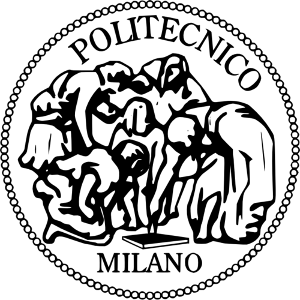
\includegraphics[width=0.30\textwidth]{./pictures/logo_poli}\par
	\vspace{1.8cm}
	{\Large {Internet of Things - 089073} \par}
	\vspace{1.2cm}
	{\LARGE \textbf{Home Automation and Monitoring} \par}
	\vspace{2.5cm}
	\begin{flushright}
		{\Large\itshape{Angelo Claudio Re \\ Giovanni Scotti \\}
		\vspace{0.5cm} 
		\Large{\textbf{Professor:} Matteo Cesana}
	    \par}
	\end{flushright}
	\vspace{2cm}
	\vfill
	% Bottom of the page
	{\large Academic Year 2017/2018 \par}
	\vspace{0.3cm}
	{\large Document version: 1.0\par}
\end{titlepage}

%Make the table of contents
\tableofcontents

%INTRODUCTION
\chapter{Introduction}
\label{ch:Introduction}
%\section{Purpose}
This document is intended to describe a \textit{Home Automation and Monitoring} system, its electronic components as well as its constraints and the interaction with the real world and the user by providing a useful work environment example.

The documentation is full of diagrams, pictures and schematics to let the final user easily implement the system itself and take advantage of its countless features.

This document is mainly addressed to computer scientists, IoT enthusiasts, makers and anyone, with some electronics and programming skills, who wants to keep an eye on his/her home and to control devices remotely.

\section{Scope}
The \textit{Home Automation and Monitoring} system aims to offer a smart solution to home automation and monitoring needs. It is intended for those kind of users who want to visualize information about their home, such as temperature or humidity, and control devices remotely.

The system consists mainly of:
\begin{itemize}
	\item a \textit{back-end}, which is in charge of managing MQTT messaging protocol as message broker and running Node-RED. It gathers data coming from boards provided with sensors and actuators and send them to a remote service provider to store information into the cloud and to open up further analysis.
	
	\item a \textit{front end}, which offered by Node-RED itself through a user-friendly and web-accessible dashboard that can be easily reached from any device connected to the same network or to the Internet by means of port forwarding.
\end{itemize}

\noindent
The system must be secure. This is why authentication is required in order to access the dashboard.
Moreover, MQTT must be secured too and clients provide credentials to the broker to join the network.
Last but not least, power consumption has been taken into account: battery-powered boards can enter a deep sleep state after publishing data.

\section{Definitions, Acronyms, Abbreviations}

\begin{itemize}
	\item \textbf{AP:} wireless Access Point, it allows Wi-Fi devices to connect a to wired network. Usually it is an integral component of routers for home or office use.
	\item \textbf{Back-end:} any device or computer program that remains in the background and offers application logic and communication interfaces to work with the front-end counterpart. It can provide a data access layer.
	\item \textbf{Front-end:} any part of a system the users directly interact with. It provides the so called presentation layer.
	\item \textbf{IoT:} Internet Of Things.
	\item \textbf{MQTT:} Message Queuing Telemetry Transport is a publish-subscribe messaging protocol.
\end{itemize}

%\chapter{}
%\label{ch:}
%\input{./original_functioning.tex}

%\chapter{}
%\label{ch:}
%\input{./implementation.tex}

%...

\end{document}